
\documentclass[oneside,numbers,spanish]{ezthesis}
\usepackage{lastpage}
\usepackage{algorithmic,algorithm}
\usepackage{pdfpages}

%% # Datos del documento #
%% Nota que los acentos se deben escribir: \'a, \'e, \'i, etc.
%% La letra n con tilde es: \~n.


%% # M'argenes del documento #
%% 
%% Quitar el comentario en la siguiente linea para austar los m'argenes del
%% documento. Leer la documentaci'on de "geometry" para m'as informaci'on.

\geometry{top=25mm,bottom=25mm,inner=25mm,outer=25mm}

%% El siguiente comando agrega ligas activas en el documento para las
%% referencias cruzadas y citas bibliogr'aficas. Tiene que ser *la 'ultima*
%% instrucci'on antes de \begin{document}.
\hyperlinking
\begin{document}

%% En esta secci'on se describe la estructura del documento de la tesis.
%% Consulta los reglamentos de tu universidad para determinar el orden
%% y la cantidad de secciones que debes de incluir.

%% # Portada de la tesis #
%% Mirar el archivo "titlepage.tex" para los detalles.

\includepdf[pages=-]{portada}

%% # Prefacios #
%% Por cada prefacio (p.e. agradecimientos, resumen, etc.) crear
%% un nuevo archivo e incluirlo aqu'i.
%% Para m'as detalles y un ejemplo mirar el archivo "gracias.tex".

\section*{Hoja de datos del jurado}

\begin{center}
\begin{tabular}{|l|}

  \hline 
  \textbf{ 1. Datos del alumno}\\ Laguna \\Rueda\\Carlos Abraham\\53 42 27 49\\
  Universidad Nacional Aut'onoma de M'exico\\Facultad de Ciencias\\Ciencias de la Computaci'on\\
  303088682  \tabularnewline
  \hline
  \textbf{2. Datos del tutor}\\ Dr. Antonio\\Capella\\Kort\tabularnewline
  \hline    
  \textbf{3. Datos del Sinodal 1}\\ Dr. Elisa\\Viso\\Gurovich\tabularnewline
  \hline 

  \textbf{4. Datos del Sinodal 2}\\ Dr. Jos'e de Jesus\\Galaviz\\Casas\tabularnewline
  \hline 
  \textbf{5. Datos del Sinodal 3}\\Lic. Francisco\\Solsona\\Cruz \tabularnewline
  \hline 
  \textbf{6. Datos del Sinodal 4}\\ Lic. Jos'e Luis\\Torres\\Rodr'iguez\tabularnewline
  \hline
  \textbf{7. Datos del trabajo escrito}\\
  Implementaci'on de un modelo de estimaci'on de precipiaci'on pluvial \\
   \pageref{LastPage} p'aginas\\2011\tabularnewline
  \hline
\end{tabular}
\end{center}


\thispagestyle{empty}
\newenvironment{dedication} {\cleardoublepage
\thispagestyle{empty}
\vspace*{\stretch{1}} \begin{center} \em} {\end{center}
\vspace*{\stretch{3}} \clearpage}
\begin{dedication}
\hfill \
\parbox{10cm}{
\begin{verse}
A alguien importante para ti
\end{verse}
}
\end{dedication}
%% # 'Indices y listas de contenido #
%% Quitar los comentarios en las lineas siguientes para obtener listas de
%% figuras y cuadros/tablas.

\tableofcontents
%\listoffigures
%\listoftables

%% # Cap'itulos #
%% Por cada cap'itulo hay que crear un nuevo archivo e incluirlo aqu'i.
%% Mirar el archivo "intro.tex" para un ejemplo y recomendaciones para
%% escribir.
\chapter{Introducci'on}
\section{Antecedentes}

En los 'ultimos 50 a\~nos la posibilidad de observar la tierra desde el espacio
nos ha brindado la oportunidad de cambiar nuestra percepci'on sobre los sistemas 
meteorol'ogicos. Especialmente con el desarrollo de sat'elites geoestacionarios 
la capacidad de observar estos fen'omenos y su evoluci'on inici'o una nueva era en 
el trabajo cient'ifico. En un principio, el simple hecho de poder observar los fen'omenos
fue un gran paso, con el tiempo la comunidad científica empez'o a trabajar en extraer informaci'on
cuantitativa de estas nuevas herramientas.

A principios de la d'ecada de 1960 los datos meteorol'ogicos, hidrol'ogicos y oceanogr'aficos
provenientes de sat'elites empezaron a tener un mayor impacto en el an'alisis del medio 
ambiente. El 7 de Diciembre de 1966, la \textit{National Aereonautics and Space Administration} (NASA)
puso en 'orbita el primer sat'elite geoestacionario \textit{Applications Technology Satellite} (ATS-1),
que ten'ia la capacidad de observar sistemas meteorol'ogicos en proceso. El sat'elite ATS-1 era
capaz de tomar una im'agen completa de la tierra cada media hora.

Poco tiempo despu'es, la \textit{National Oceanic and Atmospheric Administration} (NOAA) inici'o la
operaci'on de la serie GOES con el lanzamiento de GOES-1, llevando la
investigaci'on y monitorero del clima al siguiente nivel. 


\section{Objetivo General}
Estimaci'on de precipitaci'on pluvial en el sur de M'exico empleando
t'ecnicas que se basan en datos satelitales geoestacionarios y en
correcciones a las mismas por medio de lecturas pluviales en tierra.

\section{Objetivos particulares}
\begin{itemize}
 \item Obtener la informaci'on satelital y de las estaciones
   pluviom'etricas en tierra para espacios temporales en donde es 
conocido que ocurrieron eventos importantes de inundaciones.
 \item Dise\~nar una base de datos geogr'afica que permita acceder a la informaci'on de manera eficiente.
 \item Desarrollar un programa en C++/Fortran que se conecte a la base de datos y procese la informaci'on para obtener
un mapa de lluvias as'i como un an'alisis de los datos obtenidos para saber que tan confiable es el algoritmo.
 \item Desarrollar una p'agina web que permita a los investigadores
   acceder y ejecutar el programa de manera sencilla y amigable.
\end{itemize}

\chapter{Desarrollo}

\section{Obtener datos satelitales y lecturas \\ pluviom'etricas}

  La  \textit{National Oceanic and Atmospheric Administration} (NOAA) es una agencia federal Estadounidense que se encarga de 
  monitorear las condiciones oce'anicas y atmosf'erica por medio de sus sat'elites.
  En particular, los sat'elites geoestacionarios GOES 11 y 12 toman imagenes en infrarrojo de las nubes que est'an sobre
  el territorio Mexicano.

  Para 'este proyecto pedimos a la NOAA que nos proporcionara informaci'on de una zona amplia del sur del pa'is en 
  intervalos de tiempo, en los cuales, se presentaron fen'omenos de importancia de inundaciones en la zona de Tabasco.

  Es necesario que se procese la informaci'on que se descarga directamente de los servidores de la NOAA. Para ello se usa
  una aplicaci'on llamada \textit{NOAAA Weather and Climate Toolkit} para generar archivos de texto plano que contiene
  toda la informaci'on de cada punto le'ido.

  \begin{figure}[h!]
  \centering
  \includegraphics[width=150mm]{./imagenes/archivoTxt.png}
  % archivoTxt.png: 721x512 pixel, 72dpi, 25.43x18.06 cm, bb=0 0 721 512
  \caption{Archivo de informaci'on satelital en texto plano}
  \end{figure}


  La \textit{Comisi'on Federal de Electricidad} (CFE) posee una serie de estaciones de medici'on pluviom'etricas que registran 
  la lluvia que cae sobre la estaci'on en cada hora. El portal de la CFE permite acceder a las estaciones deseadas 
  y a las fechas disponibles. Desafortunadamente, la informaci'on que provee la CFE es limitada para algunas fechas.




\section{Dise\~no de la apliaci'on en C++/Fortran}
  %Porque se decidio usar C y Fortran
  Las aplicaciones que realizan c'alculos num'ericos complejos requieren que la velocidad de respuesta sea la m'inima posible y que
  la programaci'on de las mismas sea sencilla.

  Hist'oricamente, Fortran ha servido al mundo cient'ifico para modelar sistemas complejos. Su sint'axis, 
  muy similar al lenguaje matem'atico, lo hace sumamente atractivo para desarrollar aplicaciones num'ericas. Sin embargo,
  es su alta especializaci'on lo que permite al compilador hacer optimizaciones eficientes en el c'odigo, produciendo
  programas muy r'apidos.

  Por otra parte, C/C++ es un lenguaje de prop'osito general que permite al programador trabajar en tareas que requieren
  el uso de estructuras de datos y el acceso a los servicios del sistema operativo, por ejemplo, manejar archivos, memoria y hacer 
  conexiones a bases de datos.

  La combinaci'on de ambos lenguajes se realiza mediante la definici'on de m'etodos externos de C. De 'esta manera, es posible
  usar lo mejor de 'estos lenguajes obteniendo resultados eficientes usando una programaci'on sencilla.

  %Uso de un IDE

  Los entornos de desarrollo integrados (EDI) son herramientas sumamente 'utiles en la implementaci'on de proyectos de software.
  Los EDI son aplicaciones que consisten de un editor de c'odigo, un compilador, un depurador y una interfaz gr'afica.

  Para 'este proyecto se adopt'o Netbeans\footnote{www.netbeans.org/} en su versi'on 7 pues es uno de los EDI m'as aceptados y f'aciles de usar. La integraci'on
  que posee con C y Fortran hace que la programaci'on sea f'acil.

  %uso de gitHub
  En cualquier proyecto de desarrollo de software es indispensable contar con un control de versiones del c'odigo.
  Entre las opciones existentes, se opt'o por usar GitHub\footnote{https://github.com} pues provee de una plataforma web robusta y sobre todo segura. 
  Para 'este proyecto se us'o un repositorio privado que garantiza que s'olo los colaboradores autorizados puedan ver y modificar el c'odigo.

  Finalmente, existen dos bibliotecas que son utilizadas para realizar consultas
  a bases de datos MySQL\footnote{www.mysql.com}. Una de ellas est'a implementada en C++ y la otra en C.
  Se eligi'o la biblioteca mysqlclient implementada en C por su facilidad de uso.

%Documentación usando doxygen
  \subsubsection*{Documentaci'on detallada del programa}
  La documentaci'on detallada del c'odigo se realiz'o mediante Doxygen\footnote{http://www.doxygen.org/}. 
'Esta herramienta sirve para realizar documentaci'on de programas escritos
en diferentes lenguajes de programaci'on. Al igual que en Javadoc, la documentaci'on es escrita dentro del mismo c'odigo como comentarios, de 'esta manera 
es relativamente sencillo de mantener actualizado. Doxygen permite realizar referencias cruzadas entre la documentaci'on y el c'odigo, por lo que es muy 
sencillo ver directamente el c'odigo desde la documentaci'on.

  El producto final es una p'agina web, un manual 
  que puede ser visto con el comando man de UNIX y un documento PDF que detallan cada archivo, funci'on y m'odulo usado en el sistema.
\begin{figure}[h!]
 \centering
 \includegraphics[width=150mm]{./imagenes/doxygen1.jpg}
 % doxygen1.jpg: 896x435 pixel, 72dpi, 31.61x15.35 cm, bb=0 0 896 435
\caption{P'agina web generada por Doxygen}
\end{figure}

\subsection{Estandarizaci'on de la informaci'on}
  %Mallas artificiales
  Uno de los primeros problemas al manejar la informaci'on del sat'elite fue la naturaleza misma de la informaci'on. 

  Los sat'elites GOES 11 y 12 entregan im'agenes con resoluciones diferentes y, por lo tanto, puntos 
  diferentes para la misma hora; m'as a'un, las im'agenes no presentaban necesariamente una forma regular.

  El primer paso para manejar de manera confiable la informaci'on fue realizar un pre-proceso de la misma
  de tal manera que se contara con im'agenes consistentes y regulares.

  La soluci'on adoptada fue dividir el territorio nacional en intervalos predefinidos para generar una malla regular
  a la cual se podía ajustar la informaci'on de los satélites.

  Una vez definida la malla, se subi'o su informaci'on a la base de datos para poder obtener 
  de manera din'amica los puntos que se deben considerar para cualquier pol'igono. 

  El siguiente paso fue implementar un algoritmo de interpolaci'on que tomara una im'agen satelital arbitraria y 
  ajustara su informaci'on a una malla contenedora\footnote{Algoritmo
    implementado por Adri'an Tovar}.

 Como se ilustra en la Figura 2.3, la informaci'on del sat'elite puede ser muy irregular. Para resolver el problema 
  envolvemos la im'agen en la malla e interpolamos la informaci'on. Las zonas para las cuales no hay datos disponibles
  son rellenadas de valores -1 (Se acord'o que un valor negativo para las lluvias sería un buen indicador de que no hay
  informaci'on).

  El algoritmo de interpolaci'on se describe a continuaci'on:

  \begin{enumerate}
    \item Leer informaci'on del sat'elite y construir un arreglo de
      de las filas que conforman la im'agen.
    \item Para cada punto $x$ en la malla artificial se obtienen los
      cuatro puntos de la im'agen satelital que forman el cuadil'atero
      m'as peque\~no tal que  $x$ est'a dentro del cuadril'atero.
    \item Para realizar la interpolaci'on se requieren s'olo tres
      puntos, por lo que debemos eliminar uno de los puntos del
      cuadril'atero. Un cuadril'atero induce 2 tri'angulos. Se debe
      saber dentro de qu'e tri'angulo se encuentra el punto $x$. Para
      saberlo se usa un algoritmo que determina si un punto se
      encuentra dentro de un pol'igono usando el Teorema de la curva
      de Jordan.
    \item Finalmente, teniendo el tri'angulo m'as peque\~no que
      envuelve a un punto $x$ se puede calcular la ecuaci'on de un
      plano que pasa por esos tres puntos.
  \end{enumerate}

  %%Hacer una imagen de como podría estar la imágen satelital y como se encierra dicha im'agen en una malla artificial
  \begin{figure}[h!]
  \centering
  \includegraphics[width=100mm,bb=0 0 502 388]{./imagenes/malla.jpg}
  % malla.jpg: 502x388 pixel, 72dpi, 17.71x13.69 cm, bb=0 0 502 388
  \caption{Interpolaci'on de las imagenes satelitales}
  \end{figure}

  El programa de interpolaci'on fue implementado en Fortran mientras que las subrutinas para 
  pedir la malla adecuada a la base de datos fueron implementadas en C.

\subsection{Descripci'on del argoritmo STAR}
  El algoritmo STAR\cite{star} se encarga de transformar las temperaturas registradas por los satelites y las convierte
  en una primer estimaci'on pluvial. Recibe como entrada una matr'iz de temperaturas y para cada punto $p$ de la matr'iz
  obtiene una vecindad de radio $50$ alrededor del punto. Para esta vecindad calcula la media x' y la desviaci'on estandard $\sigma$.

  Usando 'esta informaci'on se calculan dos 'indices llamados $RRn$ y $RRc$ que finalmente son utilizados por el algoritmo STAR

  \begin{algorithm}
  \caption{C'alculo del 'indice RRc}

  \begin{algorithmic}
  \IF {$temperatura \geq 201$}
	  \STATE $rrc \gets 1.1183* (100000000000.0)^(-0.036382*temperatura^{1.2})$
  \ELSE
	  
	  \STATE $rrc \gets 72$ \COMMENT{m'aximo valor de lluvia posible}
	  
  \ENDIF 
  \end{algorithmic}
  \end{algorithm}

  \begin{algorithm}
  \caption{C'alculo del 'indice RRn}

  \begin{algorithmic}
  \IF {$temperatura \geq 250$}
	  \STATE $rrn \gets 0$
  \ELSE
	  
	  \STATE $rrn \gets min(\frac{250-temperatura}{5}, 12)$ 
	  
  \ENDIF 
  \end{algorithmic}
  \end{algorithm}

  \begin{algorithm}
  \caption{Algoritmo STAR}

  \begin{algorithmic}
  \FOR{cada punto en la imagen}
      \STATE $vecindad \gets VecindadRadio50(x,y)$
      \STATE $x' \gets Promedio(vecindad)$
      \STATE $sigma \gets Desviacion(vecindad)$  
      \STATE $rrc \gets ComputarRRc((x,y).temperatura)$
      \STATE $rrn \gets ComputarRRn((x,y).temperatura)$
      \STATE $z = min(\frac{ x'-(x,y).temperatura}{sigma}, 1.5)$
      \IF { $z > 0$}
	\STATE $rr = \frac{rrc*z^2 + rrn*(1.5-z)^2}{z^2+ (1.5-z)^2}$
      \ELSE	  
	\STATE $rr = 0$   
      \ENDIF
    \ENDFOR
  \end{algorithmic}
  \end{algorithm}

Es importante mencionar que 'este proceso se ejecuta para cada lectura del sat'elite. Es posible que se tengan 3 o 4 lecturas por hora. El algoritmo 
Asimilaci'on requiere que se tenga una sola lectura por hora. Es entonces que se debi'o realizar un promedio de los archivos si se tienen dos lecturas y 
ejecutar un algoritmo trimean cuando se tengan 3 lecturas. De 'esta manera se conserva el mejor valor posible para cada hora.
El algoritmo trimean es el siguiente:
\begin{equation}
 TM=\frac{Q_1+2Q_2+Q_3}{4}
\end{equation} 

%% Algoritmo Asimilación
\subsection{Descripci'on e implementaci'on del algoritmo \\Asimilaci'on}

El algoritmo Asimilaci'on se encarga de realizar un ajuste de los
datos calculados usando el algoritmo STAR. A continuaci'on se
describe el algoritmo.

\begin{enumerate}
 \item Descargar la malla predefinida para el pol'igono solicitado por el usuario.
  \item Computar el algoritmo STAR para obtener \textbf{hasta} 3 horas previas de la que se desea calcular.
  \item Completar la informaci'on del paso anterior con -1 en donde no se encuentre informaci'on usando la malla predefinida del paso 1.
  \item Descargar las lecturas de las estaciones que se ubican dentro del pol'igono.
  \item Correr el algoritmo \textbf{Asimilaci'on-Fortran}\footnote{Algortimo implementado por Adri'an Tovar }.
  \item En caso de 'exito, subir la informaci'on nueva a la base de datos y graficarla
  \item En caso de fracaso (informaci'on insuficiente), se debe graficar s'olo la informaci'on del algoritmo STAR.
  \item Correr el an'alisis de error puntual para cada estaci'on dentro del pol'igono.
\end{enumerate}

%Falta describir el algoritmo Asimilacion-Fortran
\subsubsection*{Algoritmo Asimilaci'on-Fortran}
El algoritmo Asimilaci'on-Fortran realiza los siguientes pasos:
\begin{enumerate}
  \item Dada la informaci'on de las estaciones en tierra, es necesario
    interpolar el valor obtenido del algoritmo STAR para el mismo
    punto y as'i, obtener el error: $Eror=ValorReal-ValorSTAR$ 
  \item Se promedian los errores por unidad de lluvia. Los valores
    posibles de lluvia toman valores en el intervalo de enteros:
    $[1,75]$. Los errores son clasificados y promedidados usando este
    intervalo para generar una gr'afica entre lluvia y errores. 
  \item Usando 'esta gr'afica se ajusta una l'inea con m'inimos cuadrados
    para obtener una pendiente $m$ y una ordenada al origen $b$, el
    algoritmo establece que $m \in (-\infty , 2]$ y $b \in [-.1
        ,.5]$. \\
    El valor resultado de la asimilaci'on se calcula siguiendo
    haciendo uso de las siguientes ecuaciones:\\
    Se sabe que: $ValorAsimilacion - ValorSTAR = Error$\\
    Por otra parte $Error = ValorStar*m+b$, por lo tanto\\
    $ValorAsimilado-ValorSTAR=ValorSTAR*m+b$ \\
    Finalmente $ValorAsimilado = (m+1)ValorSTAR+b$\\
    Cuando no se puede ajustar una l'inea porque s'olo existe un
    punto entonces s'olo se suma el valor de la coordenada $x$ del
    punto, as'i: $ValorAsimilado=ValorSTAR+x(punto)$
\end{enumerate}

El principal problema con 'este algoritmo es que no es muy funcional
si no existe informaci'on de las estaciones en tierra o si las
lecturas de las estaciones entran dentro del mismo rango de lluvia
debido a que el paso 2 promedia las lecturas por unidad de lluvia.

\section{Dise\~no de la base de datos}

El dise\~no de la base de datos geogr'afica responde a una serie de requerimientos operativos:
\begin{itemize}
 \item Debe guardar cada punto en su contexto espacial y temporal.
 \item Debe guardar la informaci'on de las estaciones de la CFE en su contexto espacial y temporal
 \item Debe guardar la informaci'on de precipitaci'on en cada punto.
\end{itemize}
El dise\~no de la base de datos sigue un esquema estrella\cite{starsqueme}. El esquema estrella consta de una tabla central, tambi\'en 
llamada tabla de hechos, y una serie de tablas, tambi\'en llamadas tablas de dimesiones, que est\'an relacionadas con la tabla de hechos y la rodean 
formando una estrella. 

El esquema estrella es muy usado en la miner\'ia de datos pues es muy simple de entender y es muy veloz para acceder a los datos guardados. 
Las consultas no son complicadas desde el punto de vista del usuario final, ya que las condiciones y uniones (JOIN) necesarias s\'olo 
involucran a la tabla de hechos y a las de dimensiones (Las tablas que rodean a la tabla de hechos).

A pesar de que la miner\'ia de datos usa el esquema estrella para realizar an\'alisi multidimiensional, las caracter\'isticas mencionadas 
hacen que \'este dise\~no sea el ideal para realizar consultas a la base de datos geogr\'afica. 


\begin{figure}[h!]
 \centering
 \includegraphics[width=150mm]{./imagenes/DataBase.jpg}
 % DataBase.jpg: 651x396 pixel, 72dpi, 22.97x13.97 cm, bb=0 0 651 396
 \caption{Dise\~no de la Base de Datos Geogr'afica siguiendo un esquema estrella}
\end{figure}

El incremento en la velocidad de acceso a la informaci'on se logra mediante la aplicaci'on de 'indices en los campos en donde
se hacen las b\'usquedas m\'as frecuentes.

En \'este proyecto se relizaron \'indices sobre diferentes tablas:
\begin{itemize}
 \item 'Indice sobre el campo \textit{fecha} en la tabla \textit{LecturaTierra}  
  \item 'Indice sobre el campo \textit{fecha} en la tabla \textit{Interpoltxt}
  \item 'Indice sobre el campo \textit{fecha} en la tabla \textit{Calculo}
  \item 'Indice geogr'afico sobre el campo \textit{punto} en la tabla \textit{Estacion}
  \item 'Indice geogr'afico sobre el campo \textit{punto} en la tabla \textit{PuntosVentana}
\end{itemize}



\section{Dise\~no de la p'agina web}
%Primefaces y JSF
En la actualidad las arquitecturas de software m'as aceptadas y adoptadas en 
el desarrollo web implementan la arquitectura llamada Modelo-Vista-Controlador (MVC).

La arquitectura MVC\cite{jsf} intenta aislar tres componentes importantes en el desarrollo
de una aplicaci'on web:

\begin{itemize}
 \item \textbf{Modelo:} Administra el comportamiento y los datos de la aplicaci'on mediante peticiones (usualmente de la vista).
\item \textbf{Vista:} Permite acceder e interaccionar con el modelo mediante una interfaz f'acil de usar.
\item \textbf{Controlador: } Recibe entradas del usuario e inicia la respuesta correspondiente haciendo llamadas al controlador.
\end{itemize}

Uno de los marcos de trabajo m'as ampliamente usados que implementan la arquitectura MVC es Java Server Faces\footnote{http://www.oracle.com/technetwork/java/javaee/javaserverfaces-139869.html}
 (JSF). En JSF las peticiones del usuario son procesadas por un servidor que carga la vista apropiada, crea el 'arbol de componentes de la vista y
procesa sus eventos. El estado de los componentes de la vista son guardados al final de una petici'on s'incrona o as'incrona al servidor.

El usuario final experimenta una experiencia visual m'as eriquecedora mediante las llamadas as'incronas al servidor que atienden
respuestas en tiempo real en el momento en que se interact'ua con la aplicaci'on. El valor agregado de JSF es la existencia de otros
marcos de trabajo que incrementan la calidad visual de los componentes de la vista, tal es el caso de PrimeFaces.

La p'agina web del presente proyecto se implement'o usando JSF 
y PrimeFaces\footnote{http://www.primefaces.org/} para lograr una experiencia visual 'optima
para que la aplicaci'on sea f'acil de usar y atractiva visualmente.

\begin{figure}[!ht]
 \centering
 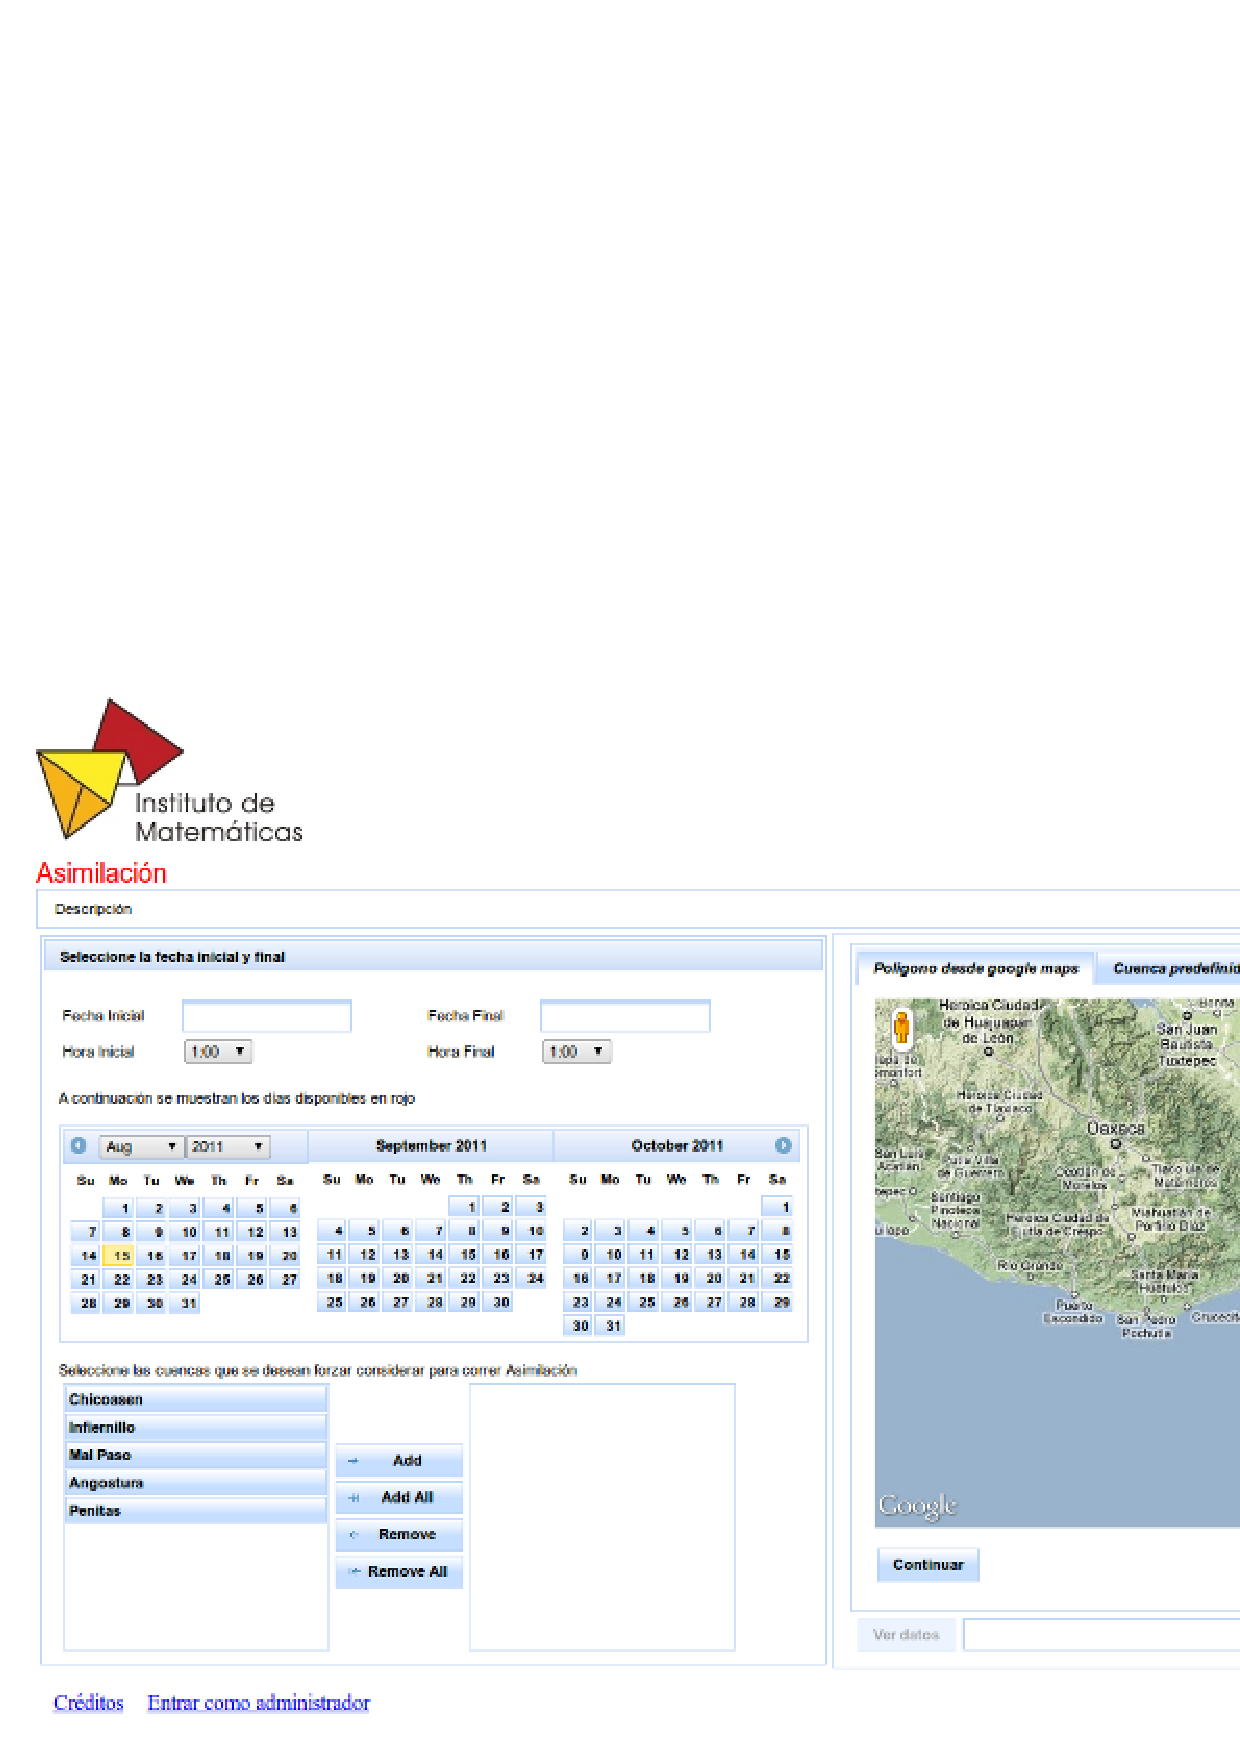
\includegraphics[width=150mm]{./imagenes/pagWeb.jpg}
 % pagWeb.png: 1425x789 pixel, 72dpi, 50.26x27.83 cm, bb=0 0 1425 789
 \caption{http://132.248.17.180:8080/AsimilacionLluvias/}
\end{figure}


La p'agina web permite seleccionar el rango de tiempo en donde se va a ejecutar el algoritmo. Se us'o Google Maps
para ilustrar la distribuci'on geogr'afica de las estaciones mediante marcas distintivas y la selecci'on de un pol'igono 
definido por el usuario.
La p'agina principal permite al usuario incluir las estaciones de cuencas disponibles para forzar que su informaci\'on 
sean considerada en la correci'on num'erica. 


\begin{figure}[ht!]
 \centering
 \includegraphics[width=150mm]{./imagenes/ejemploPagina1.jpg}
 % ejemploPagina1.jpg: 1346x564 pixel, 72dpi, 47.48x19.90 cm, bb=0 0 1346 564
 \caption{P'agina web ejecutando un c'alculo para un periodo de tiempo}
\end{figure}

\begin{figure}[h!]
 \centering
 \includegraphics[width=150mm]{./imagenes/ejemploPagina2.jpg}
 % ejemploPagina2.jpg: 1411x662 pixel, 72dpi, 49.78x23.35 cm, bb=0 0 1411 662
 \caption{P'agina mostrando el resultado del c'alculo solicitado}
\end{figure}


\section{Productos generados}
%archivo de precipitacion .debug
\subsection{Archivo de lluvia}
El programa genera un archivo con terminaci'on .debug que contiene la informaci'on calculada de las lluvias.
'Este archivo puede ser le'ido por programas de graficaci'on como gnuplot y matlab para su análisis.

En la Figura 2.8 podemos observar un ejemplo de un archivo .debug. 'Este archivo
consta de una cabecera que define las esquinas de la pol'igono y una lista de vectores (x, y, precipitaci'on). La
lista de vectores define una matr'iz regular ordenada por renglones.

\begin{figure}[h!]
 \centering
 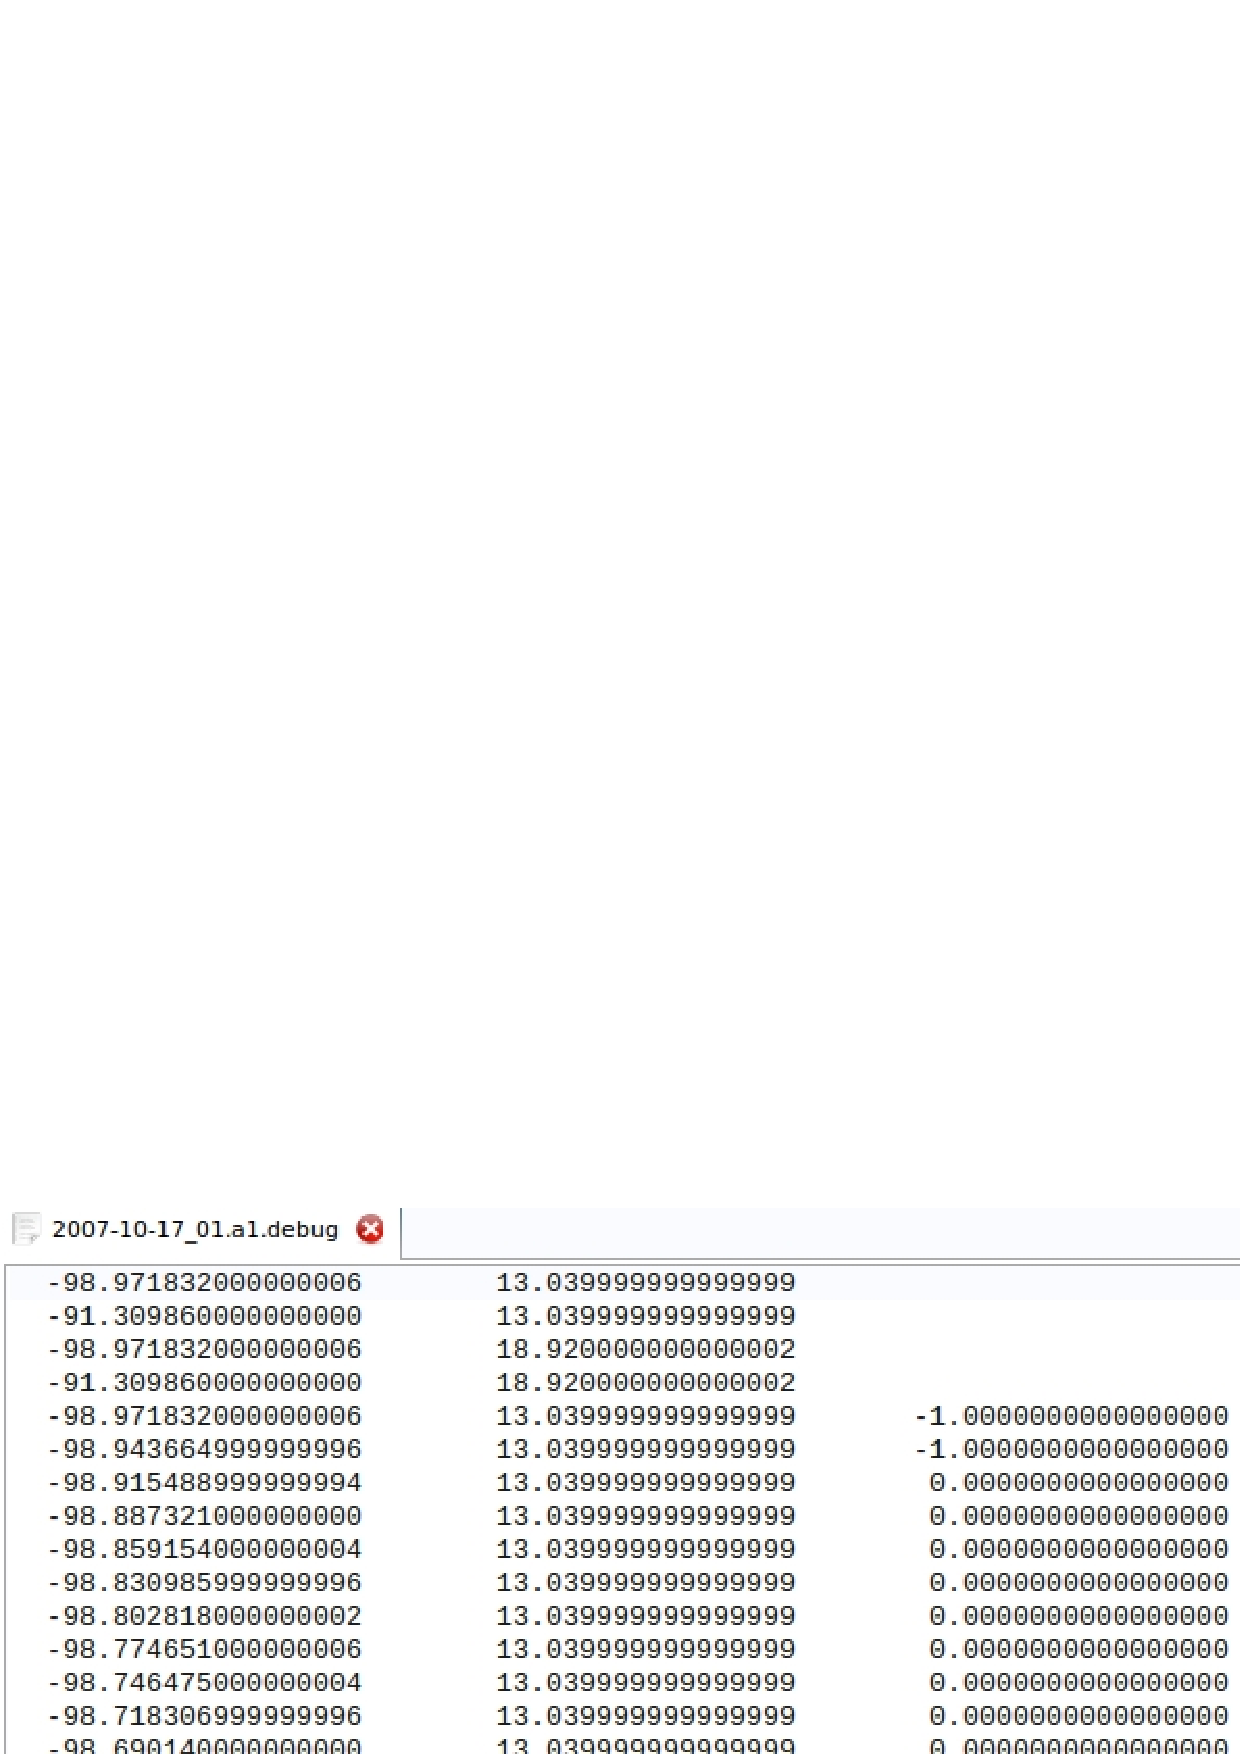
\includegraphics[width=150mm,bb=0 0 677 262]{./imagenes/archivodebug.jpg}
 % archivodebug.jpg: 677x262 pixel, 72dpi, 23.88x9.24 cm, bb=0 0 677 262
 \caption{Archivo de lluvia}
\end{figure}

\subsection{Archivo de estimaci'on puntual y pruebas de confiabilidad}
%archivo de estimaci'on puntual
El algoritmo que utiliza los valores de las estaciones de la CFE permite generar un mapa de lluvias dentro de un pol'igono
determinado. La selecci'on del pol'igono determina qu'e estaciones se deber'an usar para computar la correcci'on num'erica.

Estas premisas dan pie a analizar de manera puntual como se ha ido mejorando las estimaciones pluviales al aplicar
consecutivamente los algoritmos, es decir, mediante interpolaciones num'ericas nos fue posible comparar la precipitaci'on
real reportada por las estaciones de la CFE, contra el resultado del algoritmo STAR y el resultado de la Asimilaci'on.


El archivo de estimaci'on puntual describe el comportamiento de los 2 algoritmos de estimaci'on pluvial y los compara
contra la precipitaci'on real reportada por las estaciones de la CFE.

El archivo de estimaci'on puntual es un archivo .csv que contiene los siguientes campos por estaci'on: 
\textbf{Nombre de la estaci'on, longitud, latitud , Valor real, Valor rain rate, Valor asimilado}


\begin{figure}[h!]
 \centering
 \includegraphics[width=150mm,bb=0 0 837 507]{./imagenes/archivoErrorAnalysis.png}
 % archivoErrorAnalysis.jpg: 837x507 pixel, 72dpi, 29.53x17.89 cm, bb=0 0 837 507
 \caption{Diagrama de dispersi'on}
\end{figure}

En la figura 2.9 se muestra un diagrama de dispersi'on de las predicciones realizadas en cada paso ejecutado por el sistema.
En el eje ${y}$ se representa la precipitaci'on en una hora en particular, 
en el eje $x$ son representadas las estaciones que caen dentro de un pol'igono
determinado. 


%archivo de error sigma desv esta
\subsection{Mapas de lluvia}

Para poder presentar una im'agen de la estimaci'on pluvial probamos diferentes programas de graficaci'on, entre los cuales
destacan gnuplot\footnote{http://www.gnuplot.info/} y GrADS\footnote{http://www.iges.org/grads/}.

Se eligi'o usar GrADS, dise\~nado originalmente por \textit{ NASA Advanced Information Systems Research Program}, 
pues es un programa de prop'osito espec'ifico para manipular y visualizar datos generados por las Ciencias 
de la Tierra. Por otra parte, gnuplot es un programa de uso generar para graficar gran variedad de datos cient'ificos, lo cual
lo hace poco eficiente para graficar nuestra informaci'on, en particular, el uso de curvas de nivel fue privativo en tiempo
de ejecuci'on y en nivel de detalle de la im'agen.

Se puede apeciar en la Figura 2.7 que GrADS nos permite integrar la ubicaci'on y estado de las estaciones,
mostrando en rojo las aquellas que no poseen informaci'on, en verde las que si la poseen y en amarillo las que 
tienen informaci'on incompleta. Adicionalmente el graficador\footnote{M'odulo implementado por Adr'an Tovar} 
muestra la silueta de la Rep\'ublica Mexicana en negro y una escala de colores
lateral que modela la cantidad de lluvia que est\'a cayendo sobre una regi\'on espec\'ifica.

Directamente la im'agen generada por GrADS es un archivo EPS \textit{Encapsulated PostScript}, sin embargo a pesar de la buena calidad
de las im'agenes EPS, se debi'o convertir a el formato jpg para conservar la compatibilidad con los navegadores web.

\begin{figure}[h!]
 \centering
 \includegraphics[width=130mm]{./imagenes/2007_10_17_1.jpg}
 % 2007_10_17_01.eps.jpg: 719x555 pixel, 72dpi, 25.36x19.58 cm, bb=0 0 719 555
 \caption{Im'agen generada por GrADS de la ventana completa de datos}
\end{figure}

La generaci'on de im'agenes fue de vital importancia para poder notar detalles desicivos entre una cantidad enorme de datos.
El uso de im'agenes nos permiti'o observar que las im'agenes satelitales que provee la \textit{NOAA} abarcaban una zona mucho
m'as peque\~na que la que se solicit'o. La Figura 2.11 muestra una im\'agen que no posee suficiente informaci\'on

\begin{figure}[h!]
 \centering
 \includegraphics[width=130mm]{./imagenes/2007_10_17_2.jpg}
 % 2007_10_17_01.eps.jpg: 719x555 pixel, 72dpi, 25.36x19.58 cm, bb=0 0 719 555
 \caption{Im'agen generada por GrADS de la ventana completa de datos con informaci'on faltante}
\end{figure}

\include{manuales}
%\include{capitulo2}
%\include{capitulo3}
\include{conclusiones}
\begin{thebibliography}{1}
 \bibitem{starsqueme} Jiawei Han et. al. {\em Data Mining: Concepts and Techniques (The Morgan Kaufmann Series in Data Management Systems)} Elsevier, 2011.
\end{thebibliography}


\appendix
%% Cap'itulos incluidos despues del comando \appendix aparecen como ap'endices
%% de la tesis.
%\include{apendiceA}
%\include{apendiceB}
%\include{apendiceC}

%% Incluir la bibliograf'ia. Mirar el archivo "biblio.bib" para m'as detales
%% y un ejemplo.
%%\bibliography{biblio}

\end{document}
